\subsection{p < 1 bar}
Um die Verdampfungswärme L zu berechnen, wird die Formel
\begin{equation*}
  \ln \bigl(\frac{p}{p_0}\bigr)=-\frac{\symup{L}}{\symup{R}} \cdot \frac{1}{\symup{T}}
  %schon verwendet?
\end{equation*}
verwendet. Hierbei ist $p_0$ der Umgebungsdruch und beträgt
\begin{equation*}
  p_0=995\cdot 10^2 \si{\pascal}.
\end{equation*}
Die in Tabelle\ref{tab:data1} gemessenen Werte für den Druck werden logarithmiert und in eien
Diagramm gegen den Kehrwert der absoluten Temperatur aufgetragen. \\
   \begin{table}
    \centering
    \caption{Messung bis 1 bar}
    \label{tab:data1}
    \begin{tabular}{c c c c}
      \toprule
      T/°C & P/bar & T/°C & P/bar
      \\
      \midrule
      52    &   137  &  76  &  400  \\
      53    &   146  &  77  &  417  \\
      54    &   153  &  78  &  439  \\
      55    &   160  &  79  &  454  \\
      56    &   167  &  80  &  474  \\
      57    &   174  &  81  &  490  \\
      58    &   183  &  82  &  515  \\
      59    &   191  &  83  &  532  \\
      60    &   200  &  84  &  555  \\
      61    &   209  &  85  &  577  \\
      62    &   219  &  86  &  600  \\
      63    &   229  &  87  &  625  \\
      64    &   239  &  88  &  650  \\
      65    &   249  &  89  &  666  \\
      66    &   261  &  90  &  702  \\
      67    &   271  &  91  &  726  \\
      68    &   286  &  92  &  756  \\
      69    &   299  &  93  &  780  \\
      70    &   311  &  94  &  807  \\
      71    &   325  &  95  &  837  \\
      72    &   339  &  96  &  881  \\
      73    &   352  &  97  &  912  \\
      74    &   369  &  98  &  947  \\
      75    &   384  &  99  &  988  \\
      %Wert für 100°C fehlt wegen Formatierung
      \bottomrule
    \end{tabular}
  \end{table}

\begin{figure}
  \centering
  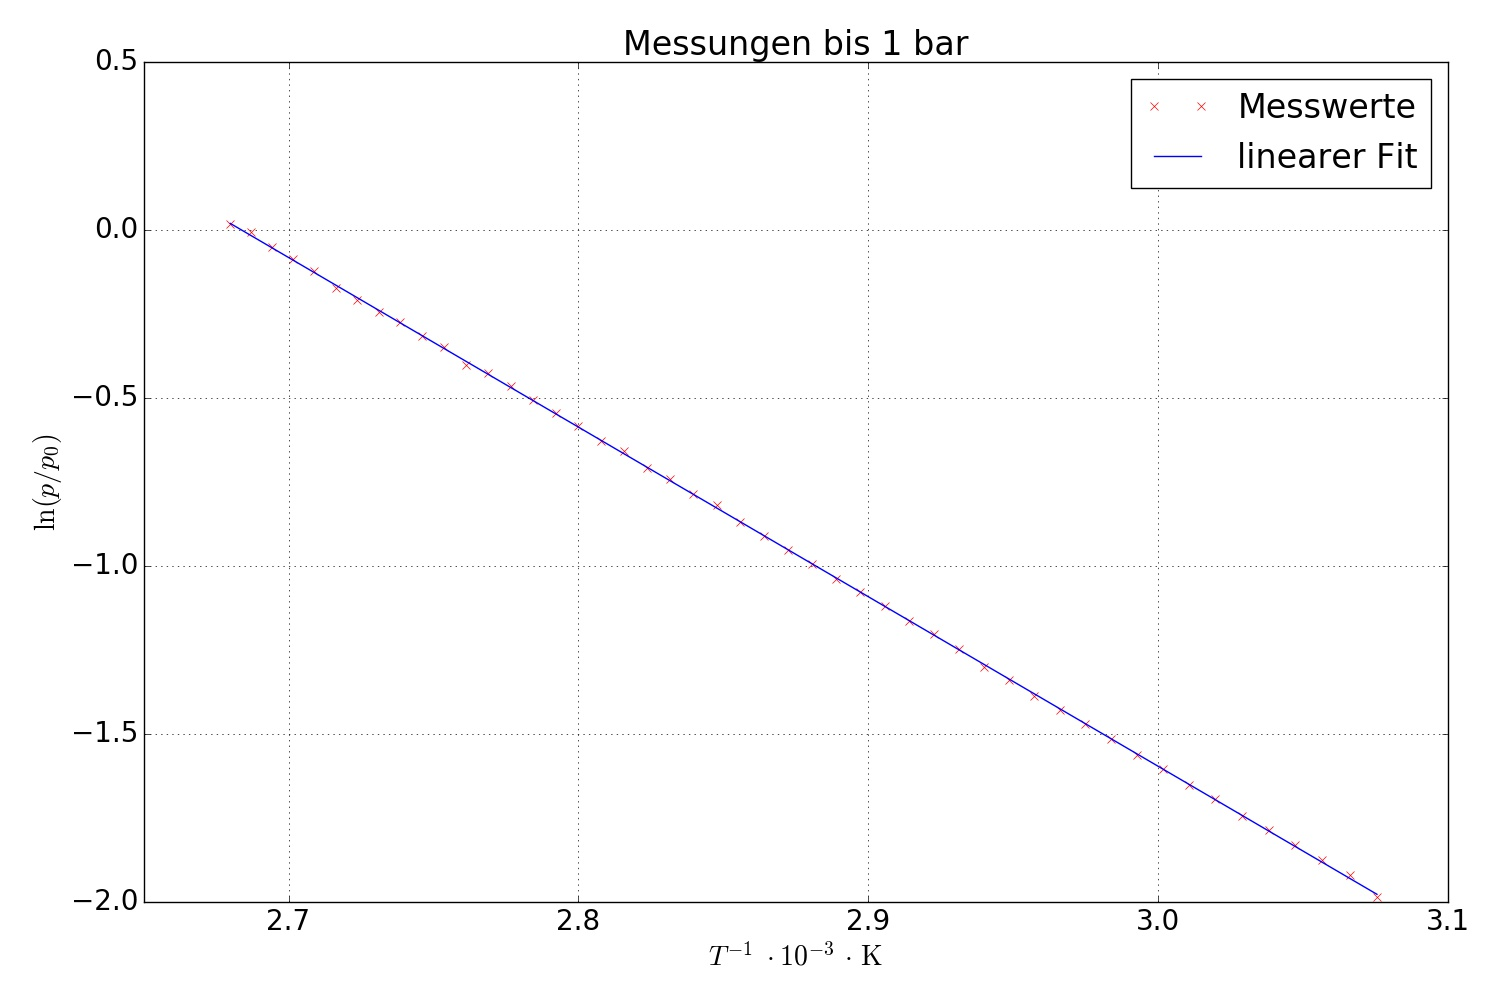
\includegraphics[height=9cm , width=13.5cm]{fit1.jpg}
  \caption{fit1}
  \label{fig:fit1}
  \end{figure}
  \\
Die Parameter der linearen Regression werden mit Python 3.5.2 berechnet und
lauten:
\begin{align*}
  a =& (-5,044 \pm 0,006) \cdot 10^3 \si{\kelvin} \\
  b =& (13,537 \pm 0,169)
\end{align*}
unter Verwendung von Formel \eqref{eq:4} und der allgemeinen Geradengleichung
lässt sich L mit
\begin{equation}
  a=-\frac{L}{\symup{R}} \iff L = -a \cdot \symup{R}
\end{equation}
darstellen. Der dazugehörige Fehler wird über die Gaußsche Fehlerfortpflanzung
berechnet und liefert:
\begin{equation}
  \Delta f = \sqrt{-\symup{R}^2 \cdot \Delta a^2}.
\end{equation}
Wobei R die allgemeine Gaskontante und $\Delta a$ der Fehler von $a$ ist.
Somit ist:
\begin{equation*}
  L=(41,938 \pm 0,050)\cdot 10^3 \frac{\si{\joule}}{\si{\mol}}.
\end{equation*}
\newpage
Weiter soll die äußere Verdampfungswärme $L_a$, also die Energie, welche
benötigt wird um das Volumen der Flüssigkeit auf das Volumen des Gases
zu bringen. Hierbei wird eine Volumenarbeit $W=pV$ geleistet.
Über gleichsetzen der idealen Gasgleichung \eqref{eq:ideal} mit der
Volumenarbeit, lässt sich $L_a$ für eine Temperatur von $T=373 \si{\kelvin}$
berechnen:
\begin{align*}
  L_a =& W =pV=RT \\
      =& 3,101 \cdot 10^3 \si{\joule \per \mol}
\end{align*}
Die innere Energie $L_i$ muss aufgebracht werden, um die molekularen
Anziehungskräfte zu überwinden. Diese ist
\begin{align*}
  L_i=&L-L_a \\
  =& (38,837 \pm 0,050)\cdot 10^3 \si{\joule\per\mol}.
\end{align*}
 Die innere Energie pro Molekül erhält man Division mit der Avogadrokonstanten
 $\symup{N_A}=6,022 \cdot 10^{23} \frac{1}{\si{\mol}}$.
 Dieses Ergebnis wird der Anschaulichkeit halber in Elektronenvolt angegeben
 ($1\si{\electronvolt}=1,602\cdot 10{{-19}}\si{\joule})$.
 Der Fehler wird erneut über die Gaußsche Fehlerfortpflanzung berechnet:
 \begin{equation*}
   \Delta f=\sqrt{\frac{1}{\symup N_A^2}\cdot 0,050^2}.
 \end{equation*}
 somit:
 \begin{equation*}
   L_i=4,025\cdot 10^{-4} \pm 5,182\cdot 10^{-7}\si{\electronvolt}
 \end{equation*}
\subsection{Messungen bis 15 bar}
Hier kann man dann mit Tabelle 2 weiter machen:
\begin{table}
  \centering
  \caption{Messung bis 15 bar}
  \label{tab:data2}
\begin{tabular}{c c c c}
  \toprule
  T/\si{\celsius} &   P/\si{\bar}  &   T/\si{\celsius} &   P/\si{\bar} \\
  \midrule
  100  &   2.24   &   132  &   4.69  \\
  102  &   2.33   &   134  &   4.94  \\
  104  &   2.43   &   136  &   5.20  \\
  106  &   2.54   &   138  &   5.48  \\
  108  &   2.66   &   140  &   5.78  \\
  110  &   2.78   &   142  &   6.11  \\
  112  &   2.90   &   144  &   6.48  \\
  114  &   3.04   &   146  &   6.87  \\
  116  &   3.18   &   148  &   7.31  \\
  118  &   3.34   &   150  &   7.79  \\
  120  &   3.50   &   152  &   8.36  \\
  122  &   3.67   &   154  &   9.03  \\
  124  &   3.85   &   156  &   9.81  \\
  126  &   4.04   &   158  &  10.86  \\
  128  &   4.25   &   160  &  12.26  \\
  130  &   4.47   &   162  &  14.46  \\
  \bottomrule
  \end{tabular}
\end{table}
 \\
Hier geht die Auswertung dann Normal weiter
